\documentclass[10pt,a5paper]{article}
\renewcommand{\baselinestretch}{1.0}
\usepackage{cite}
\usepackage[dvips]{graphicx}
\usepackage{psfrag}
\usepackage{color}
\usepackage[cmex10]{amsmath}
\usepackage{amsfonts}
\usepackage[font=footnotesize, captionskip=10pt]{subfig}
\usepackage{tikz}
\usepackage{flushend}
\usepackage{times}
\usepackage[margin=1.5cm]{geometry}

\usepackage[slovak]{babel}
\usepackage[utf8]{inputenc}
\usepackage[T1]{fontenc}

\pagestyle{empty}

\hyphenation{net-works}
\newtheorem{remark}{Remark}

\begin{document}

\title{About cross synaptic neuron model}
\author{Michal Chovanec\\
michal.chovanec@yandex.com}
\date{}
\maketitle
\thispagestyle{empty}

%\noindent$^1$\ affiliation\\
%\noindent$^2$\ affiliation\\

\noindent {\bf Keywords:} neural network, neuron model, modification

\noindent {\bf Abstract:} In this paper, experimental neuron model with ability
multiply inputs is described. Many tests an comparsion with other common models
has been processed on funcion aprxoimation problem.

\section{Introduction}

Well know McCulloch Pitts neuron model

\begin{equation}
\label{eq:McCulloch_Pitts}
  y(n) = \varphi(\sum_{i = 0}^{N-1} x_i(n)w_i(n))
\end{equation}

where \\
$x(n)$ is input vector \\
$y(n)$ is neuron output \\
$w(n)$ is weight vector \\
$\varphi(t)$ is neuron transfer function. \\

Common used transfer functions are (citovat) \\
linear $\varphi(t) = t$ \\
tanh $\varphi(t) = tanh(t)$ \\
step $\varphi(t) = sgn(t)$ \\

very popular is also rectified neuron model $\varphi(t) = max(0, t)$

Multilayer neural network using this model can be used as universal function aproximator \cite{bib:Aproximation}. Usually
many hidden layers need to be used, which is dificult to learn using backpropagation
algorithm - local minima.

\section{Proposed model}

We define following neuron model with ability to multiply two signals
\begin{equation}
\label{eq:testing_neuron}
  y(n) = \varphi( \sum_{i = 0}^{N-1} x_i(n)w_i(n) + \sum_{j = 0}^{N-1}\sum_{i = j}^{N-1} x_i(n)x_j(n)v_{ji}(n) )
\end{equation}

where $v_{ji}$ is matrix representing weights for multiplied inputs.

For learning process we can use common backpropagation algorithm
\begin{equation}
\label{eq:testing_neuron_learning}
    \delta w_i(n) = \eta e(n) x_i(n)
\end{equation}

\begin{equation}
\label{eq:testing_neuron_back}
    e_i(n) = w_{j i}(n) e_j(n) \varphi ' (y_j(n))
\end{equation}

For our experiments linear and tanh transfer function has been used, when linear transfer function
is used, we can write

\begin{equation}
\label{eq:testing_neuron_back_lin}
    e_i(n) = w_{j i}(n) e_j(n)
\end{equation}

and finally for tanh

\begin{equation}
\label{eq:testing_neuron_back_tanh}
    e_i(n) = w_{j i}(n) e_j(n) y_j(n)(1 - y_j(n))
\end{equation}


\section{Experimental results}

yeah, fucking awesome, many pictures == many pages to be taken

\begin{figure}[!ht]
\centering
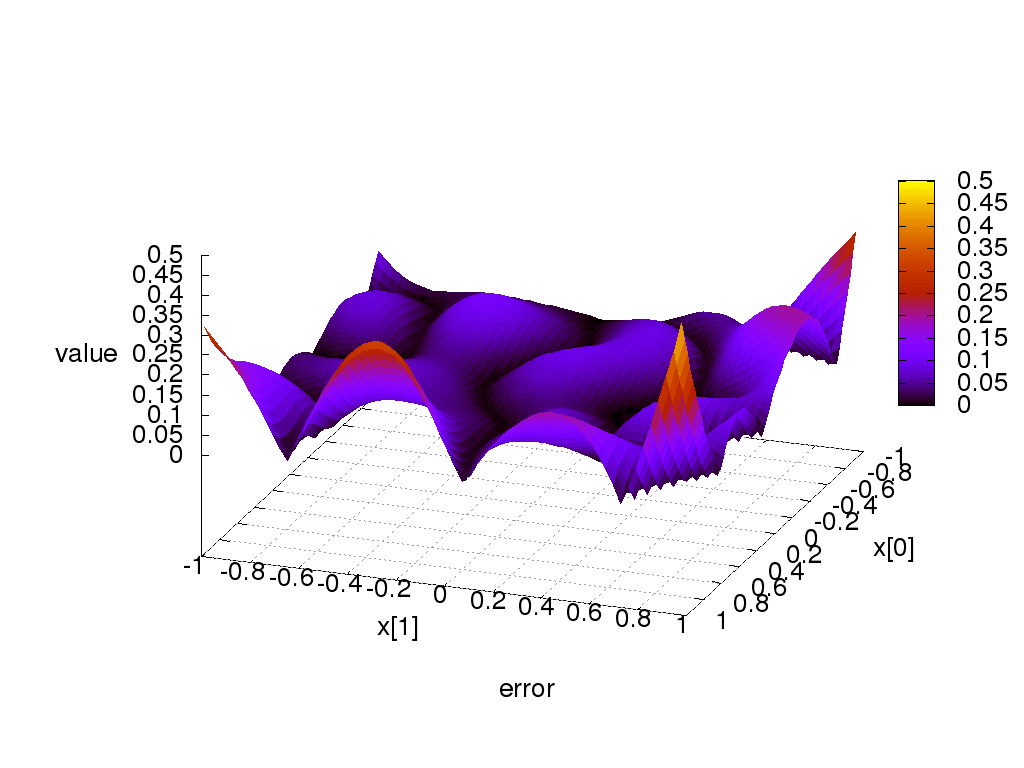
\includegraphics[width=3.0in]{pictures/results/mcculloch_pitts_neuron_1_layer/experiment_2/result_log_error.png}
\caption{experiment schematic}
\label{experiment schematic}
\end{figure}

\subsection{Experiment 1}



\section{Zaver}


\bibliographystyle{IEEEtran}
\bibliography{bib}

\begin{thebibliography}{4}

\bibitem{bib:Aproximation} Kolmogorov's Theorem,
http://neuron.eng.wayne.edu/tarek/MITbook/chap2/2\_3.html


\end{thebibliography}



\end{document}
